%  LaTeX support: latex@mdpi.com
%  In case you need support, please attach any log files that you could have, and specify the details of your LaTeX setup (which operating system and LaTeX version / tools you are using).

%=================================================================

\documentclass[remotesensing,article,accept,moreauthors,pdftex,12pt,a4paper]{mdpi} 
%--------------------
% Class Options:
%--------------------
% journal
%----------
% Choose between the following MDPI journals:
% actuators, administrativesciences, aerospace, agriculture, agronomy, algorithms, animals, antibiotics, antibodies, antioxidants, appliedsciences, arts, atmosphere, atoms, axioms, behavioralsciences, bioengineering, biology, biomedicines, biomolecules, biosensors, brainsciences, buildings, cancers, catalysts, cells, challenges, chemosensors, children, chromatography, climate, coatings, computation, computers, cosmetics, crystals, dentistryjournal, diagnostics, diseases, diversity, econometrics, economies, education, electronics, energies, entropy, environmentalsciences, environments, fibers, foods, forests, futureinternet, galaxies, games, genes, geosciences, healthcare, humanities, informatics, information, inorganics, insects, ijerph, ijfs, ijms, ijgi, jcdd, jcm, jdb, jfb, joi, jlpea, jmse, jpcg, jpm, jrfm, jsan, land, laws, life, lubricants, machines, marinedrugs, materials, mathematics, medicalsciences, membranes, metabolites, metals, microarrays, micromachines, microorganisms, minerals, molbank, molecules, nanomaterials, ncrna, nutrients, pathogens, pharmaceuticals, pharmaceutics, pharmacy, photonics, plants, polymers, processes, proteomes, publications, religions, remotesensing, resources, risks, robotics, sensors, socialsciences, societies, sports, sustainability, symmetry, systems, technologies, toxics, toxins, vaccines, veterinarysciences, viruses, water
%---------
% article
%---------
% The default type of manuscript is article, but could be replaced by using one of the class options: 
% article, review, communication, commentary, bookreview, correction, addendum, editorial, changes, supfile, casereport, comment, conceptpaper, conferencereport, meetingreport, discussion, essay, letter, newbookreceived, opinion, projectreport, reply, retraction, shortnote, technicalnote, creative
%----------
% submit
%----------
% The class option "submit" will be changed to "accept" by the Editorial Office when the paper is accepted. This will only make changes to the frontpage (e.g. the logo of the journal will get visible), the headings, and the copyright information. Journal info and pagination for accepted papers will also be assigned by the Editorial Office.
% Please insert a blank line is before and after all equation and eqnarray environments to ensure proper line numbering when option submit is chosen
%------------------
% moreauthors
%------------------
% If there is only one author the class option oneauthor should be used. Otherwise use the class option moreauthors.
%---------
% pdftex
%---------
% The option "pdftex" is for use with pdfLaTeX only. If eps figure are used, use the optioin "dvipdfm", with LaTeX and dvi2pdf only.

%=================================================================
\setcounter{page}{1}
\lastpage{x}
\doinum{10.3390/------}
\pubvolume{xx}
\pubyear{2021}
\history{Received: xx / Accepted: xx / Published: xx}
%------------------------------------------------------------------
% The following line should be uncommented if the LaTeX file is uploaded to arXiv.org
%\pdfoutput=1

%=================================================================

% Add packages and commands to include here
% The amsmath, amsthm, amssymb, hyperref, caption, float and color packages are loaded by the MDPI class.
%\usepackage{graphicx}
%\usepackage{subfigure,psfig}


\usepackage[margins]{trackchanges}
%%     \add[editor]{text to add}
%%     \remove[editor]{text to remove}
%%     \change[editor]{text to remove}{text to add}
%%     \annote[editor]{text to annotate}{note}
%%     \note[editor]{note}
%% Editors for color coding in track changes
\addeditor {peter}
\addeditor {bec}




%=================================================================
%% Please use the following mathematics environments:
%\theoremstyle{mdpi}
%\newcounter{thm}
%\setcounter{thm}{0}
%\newcounter{ex}
%\setcounter{ex}{0}
%\newcounter{re}
%\setcounter{re}{0}
%\newtheorem{Theorem}[thm]{Theorem}
%\newtheorem{Lemma}[thm]{Lemma}
%\newtheorem{Characterization}[thm]{Characterization}
%\newtheorem{Proposition}[thm]{Proposition}
%\newtheorem{Property}[thm]{Property}
%\newtheorem{Problem}[thm]{Problem}
%\newtheorem{Example}[ex]{Example}
%\newtheorem{Remark}[re]{Remark}
%\newtheorem{Corollary}[thm]{Corollary}
%\newtheorem{Definition}[thm]{Definition}
%% For proofs, please use the proof environment (the amsthm package is loaded by the MDPI class).

%=================================================================

% Full title of the paper (Capitalized)
\Title{Estimating Fractional Cover Using a Multilayer Perceptron}

% Authors (Add full first names)
\Author{Peter Scarth $^{1,}$* and Rebecca Trevithick$^{2}$}

% Affiliations / Addresses (Add [1] after \address if there is only one affiliation.)
\address{%
$^{1}$ Joint Remote Sensing Research Program, The University of Queensland, Brisbane, QLD 4072, Australia\\
$^{2}$ Joint Remote Sensing Research Program, Department of Science and Environment (DES), 41 Boggo Road, Dutton Park 4102, Australia}

% Contact information of the corresponding author (Add [2] after \corres if there are more than one corresponding author.)
\corres{p.scarth@uq.edu.au, +61439744397}

% Abstract (Do not use inserted blank lines, i.e. \\) 
\abstract{This research builds a machine learning model to derive fractional cover from moderate spatial resolution imagery by optimising a multilayer perceptron using 4000 field measurements of fractional cover over the Australian landscape. The widely used sum to one and positivity constraints are incorporated using a novel loss function. This model produces a reasonably accurate continental scale fractional cover time series than can be operationally used to support land management tasks.}

% Keywords: add 3 to 10 keywords
\keyword{fractional cover, ground cover, rangelands, unmixing}

% The fields PACS, MSC, and JEL may be left empty or commented out if not applicable
%\PACS{}
%\MSC{}
%\JEL{}

\begin{document}

%%%%%%%%%%%%%%%%%%%%%%%%%%%%%%%%%%%%%%%%%%

\section{Introduction}



Vegetation cover is variable in time and space, changing in response to both climatic variation, local pressure from grazing animals and anthropogenic influence such as cropping cycles, vegetation management and fire. The measurement of vegetation cover is an essential component of natural resource management strategies in many areas. In Australia, vegetation cover is monitored at a national scale to inform models of wind and water erosion and to evaluate the effect of funded schemes designed to improve ground cover. At a local scale, regional groups and individual farmers use ground cover data derived from Landsat to assess stocking strategies and pinpoint degraded areas on the landscape rehabilitation works. Ground cover is a critical attribute of the landscape affecting infiltration, runoff, water erosion and wind erosion, and as such is a key indicator of land condition \citep{Karfs2009}. Ground cover is driven largely by climate and management \citep{Dube2001}, however, a reduction is cover does not necessarily correspond to a decline in land condition \citep{Pickup1998}. In this paper, we refer to "cover" as the proportion of green and non-green vegetation as viewed from above the tallest vegetation stratum, which may include visible ground cover. We refer to "ground cover" as being the proportion of the ground surface covered by green and non-green vegetation. It does not include the cover contributions from persistent and perennial shrubs and trees which may exist as a stratum above the ground surface.
% * <rebecca.trevithick@gmail.com> 2015-01-06T00:00:52.009Z:
%
%  ground cover focused
%
\subsection{Remote Sensing of Cover}

The measurement of cover across large spatial extents using remote sensing has been demonstrated by several authors in the past. However, for management applications, it is often useful to know not only the cover level but also the cover components of green and non-green vegetation. In most natural systems, cover can be classified into green, non-green and bare ground. Since these components ought to sum to 100\% a mixture modelling approach, where a pixel reflectance is assumed to be a linear combination of the proportional area of each cover type, is a suitable model. There are many examples of spectral unmixing to look at cover components. Early work by \citep{Pech1986a} used image derived endmembers representing 'cover' and 'greenness' to map proportional cover types and landscape components across a rangeland. These methods were extended by \citep{Pickup1998} to look at grazing gradients and their changes over time. By extending the concept of cover in rangeland environments to include in photosynthetic vegetation (PV), non-photosynthetic vegetation (NPV) and bare soil, \citep{Harris2003} showed how imaging spectroscopy can be used to detect fine scale spatial variations in cover that can be used to assess condition. By quantifying at the spatial and temporal variation in these components \citep{Roeder2007} developed an indirect indicator of land degradation. More recently variable endmember methods such as those used by \citep{Roberts1998} have proven to be successful, particularly in complex urban environments. However these bundle methods fail in rangeland environments due to the similarity between senescent cover and bright soils \citep{Asner2002}, and the similarity between shade and dark soil since the method is unable to determine if and how much of the shade component is present within a pixel \citep{Okin2001}. Endmember bundles to accommodate the similarities have been shown to have a near singular mixture matrix in this results in poor estimates of the cover components. 

\subsection{Deriving Consistent Endmembers}

All of these unmixing methods rely on having a good spectral library where the spectra is collected either in the field spectrometer or from the image itself. However, it is rare to find a pure 30 m x 30 m Landsat pixel in heterogeneous rangeland environment and the vast rangeland extents make the collection of a representative spectral library problematic. Therefore, to characterise the variability inherent in rangeland environments and define broadly applicable end members that are suitable for application over a large geographical extent, is necessary to develop methods to derive synthetic and members from field data representing impure pixels. It has been shown by several authors that in many cases a linear unmixing process is mathematically equivalent to multiple regression when an image index is derived by regressing the individual bands against field data \citep{Puyou-Lascassies1994,Settle1998}. Recent work is also shown that multiple regression techniques are very effective at estimating foliage cover across large spatial extents when the input calibration data adequately represents the variability inherent in the landscape \citep{Armston2009}. This work seeks to use multiple regression of field data against image data to derive end members that can then be used within the constrained unmixing approach. Since the regression estimates represent an optimal estimator in the training sites we can use these endmember estimates within the constrained unmixing algorithm to provide a good estimate of the cover fractions outside the training regions. 




%%%%%%%%%%%%%%%%%%%%%%%%%%%%%%%%%%%%%%%%%%

\section{Data and Methods}

\subsection{Data}

Cover can vary rapidly in space and time, due to rainfall events causing greening up and/or grazing animals moving through and eating or trampling cover. Thus the field and satellite data need to be contemporenaiously collected. Fortunately, with the advent of the complete Landsat data
% * <rebecca.trevithick@gmail.com> 2015-01-05T02:27:25.214Z:
%
%  This is an incomplete sentence
%


\subsubsection{Field Data}


Field data was collected over several campaigns lasting from February 1997 until July 2013. Sites were selected based on an analysis of land types across Australia coupled with the expert knowledge of local field officers who pinpointed appropriate target sites. The 1549 target sites were located in both homogeneous and heterogeneous environments across both grazing and cropping lands and also sampled a range of overstory tree canopies so that algorithms to remove the effect of tree canopies could be developed at a later stage. A map of field site locations is shown in \ref{fig:fieldSiteMap}.



\begin{figure}
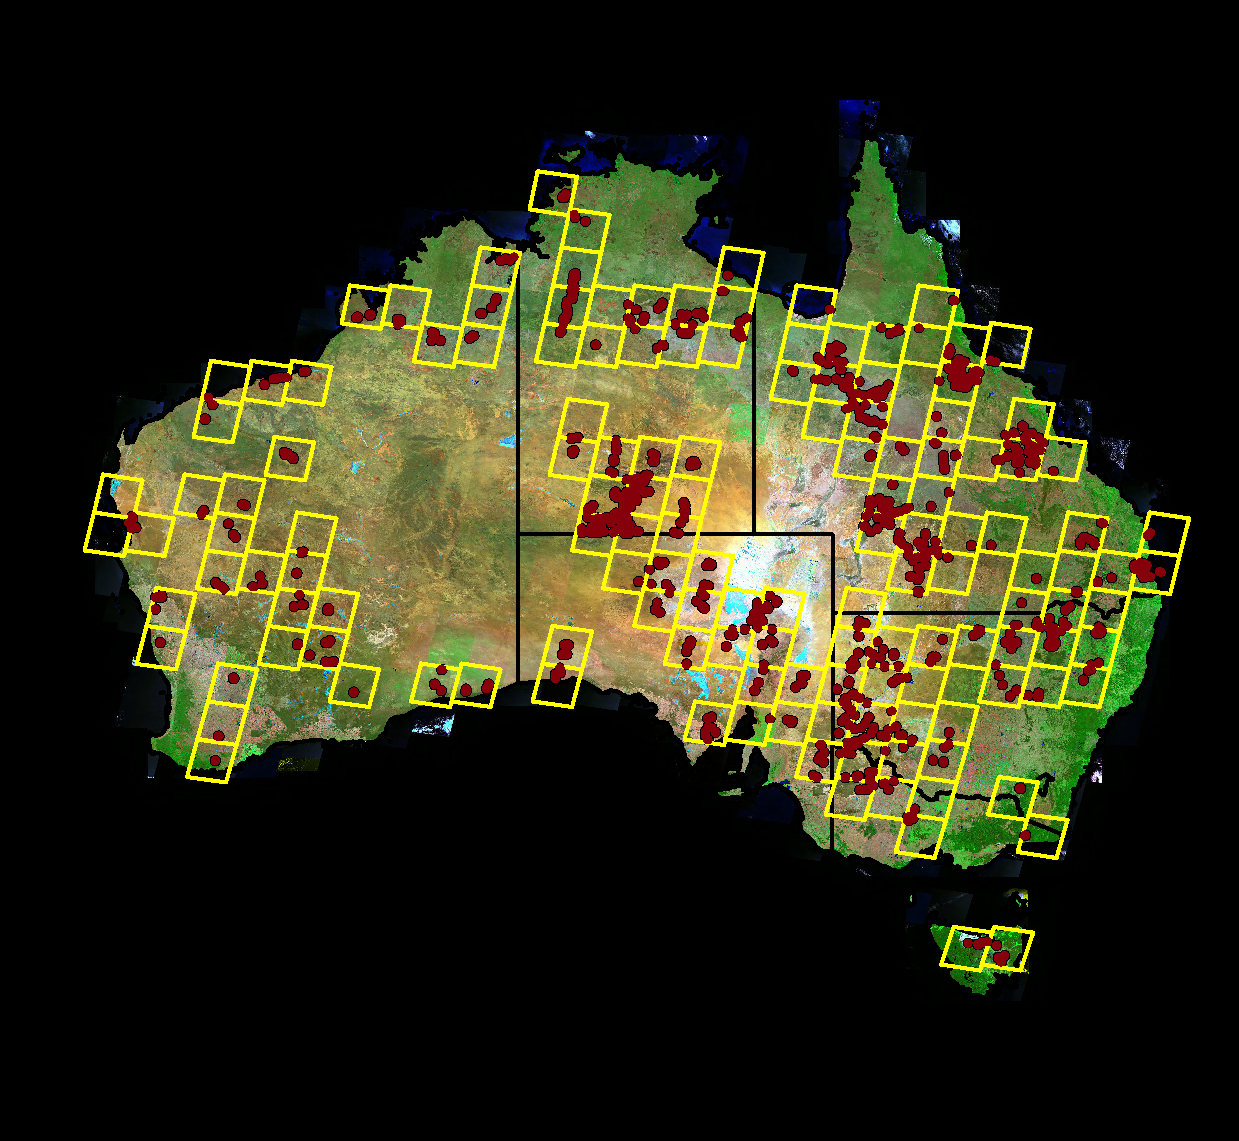
\includegraphics[width=0.5\paperwidth]{siteMap.pdf}
% * <rebecca.trevithick@gmail.com> 2015-01-05T03:40:21.337Z:
%
%  need to improve this map. points not visible, no state boundaries
%
% ^ <rebecca.trevithick@gmail.com> 2015-01-05T04:23:58.720Z.
\caption{\label{fig:fieldSiteMap} Map of Australia showing the location of field sample plots (red dots) and Landsat calibration scenes (yellow squares).}

\end{figure}


At each field site a range of measurements were taken. These can be separated into two components: Collection of discrete point transect sampling data to determine ground cover and the Foliage Projective Cover (FPC) of the overstory and midstory woody vegetation; Description of general site details, including characteristics such as soil and rock hue value and chroma, tree basal area, dominant species, and soil surface characteristics according to the method described by \citep{Muir2011}.
All cover data was collected using a discrete point sampling method consisting of  three 100-metres transects intersecting at the mid-point at 60 degree intervals from the previous transect covering an area of approximately 1 ha \citep{Muir2011}. For agricultural crops sown in parallel rows, as well as some historical transects, only two 100-metre transects positioned at 90 degrees were used. At every metre interval along these transects a recording is made of the ground cover, midstory and overstory, resulting in 200 or 300 measurements depending on the number of transects used. 
It needs to be noted that there are many other field measurement techniques that could have been utilised to measure the amount of ground cover, or its mirror, bare ground. Examples of these include, visual estimates within various size quadrats and continuous measurement along a down slope transect. The discrete point sampling technique was employed because it provided the best compromise between repeatability between different operators without requiring estimation training and regular calibration, and the time taken to measure each site in the field. 

% * <rebecca.trevithick@gmail.com> 2015-01-05T02:47:36.219Z:
%
%  This is weird. The cover elements are not itemised. Not sure what this is meant to look like
%
% ^ <rebecca.trevithick@gmail.com> 2015-01-05T03:02:25.028Z.
% * <rebecca.trevithick@gmail.com> 2015-01-05T02:41:11.104Z:
%
%  needs to be updated
%
% ^ <rebecca.trevithick@gmail.com> 2015-01-05T05:48:08.522Z.
% * <rebecca.trevithick@gmail.com> 2015-01-05T02:40:23.330Z:
%
%  probably not correct
%

\subsubsection{Image Data}

Accurate detection and quantification of vegetation change over time and space requires removal of the confounding effects of geometric distortion; radiometric variability; illumination geometry; and cloud, shadow and water contamination from imagery. These pre-processed Landsat TM and ETM data form the basis of all derived image products. A high level of automation is essential as there are over 135000 images covering the period 1987\textendash{}2013 in the RSC archive, and there is an ongoing requirement to reprocess the whole archive as improved pre-processing techniques emerge. 
% * <rebecca.trevithick@gmail.com> 2015-01-05T02:41:56.632Z:
%
%  update this 
%

Path-oriented TM and ETM+ imagery are acquired with Australian Centre of Remote Sensing Level 5 processing, which includes some systematic geometric correction and onboard radiometric calibration. Sub-pixel geometric accuracy is obtained by registering all TM and ETM+ imagery to an orthorectified ETM+ panchromatic mosaic, which is registered to Differential Global Positioning System (GPS) measured ground control points. The pre-flight radiometric calibration is used for ETM+ images; the onboard calibration is removed from TM images and an improved time-dependant vicarious calibration \citep{Vries2007}. In the future, coefficients published in \citep{Chander2009} will be adopted as they were determined from a longer time series of Landsat 5 TM imagery. Images are converted to top-of-atmosphere (TOA) reflectance and a three-parameter empirical model applied to further reduce variation in scene-to-scene illumination geometry and bi-directional reflectance distribution function (BRDF). The model, a modified version of Walthall\textquoteright{}s BRDF model \citep{Walthall1985}, was parameterized using the north-south and east-west overlapping regions of the ETM+ and TM images. Although generalized, the correction considerably reduces scene-to-scene variability.
% * <rebecca.trevithick@gmail.com> 2015-01-06T01:13:49.930Z:
%
%  Does this need updating?
%

The cross calibration between Landsat TM and Landsat ETM plus was effected through the use of a simple multiple regression technique whereby two tandem scenes (insert dates and details here) were precision rectified and then simply regressed against one another to come up with a model regression equation that converted the Landsat seven radiances back to Landsat five radiances. The blue band (Landsat band 1) was discarded in all the images due to the effects of Rayleigh scattering on shorter wavelengths. 

\subsubsection{Extraction }

Signatures for Landsat bands 1 to 7 were extracted for the 3 x 3 pixel mean surrounding the field site location. The 3 x 3 block average provided the best match to the spatial extent of field measurements and also allowed the calculation of the variance within the window. The reciprocal of the variance was used as a weighting in the regression.

Signatures were extracted from any image in the database where the field site was unnaffected by cloud or missing data and there was less then 60 days between the field measurement and the image acquisition. The number of days between field and image data was used as a weighting in the regression. This is due to the fact that cover can change extremely rapidly after rainfall events or under heavy grazing conditions and so with increasing timelag between field and image acquisition there is a great uncertainty that the field measurements accurately represent the cover conditions at the time of image acquisition. The decay function is chosen so that the weighting is approximately half after around one week. A weighting was also used to account for variation is in site heterogeneity. This accounts for the fact that as the site heterogeneity increases the certainty with which we can establish a mean cover value decreases \citep{Korb2003}.
% * <rebecca.trevithick@gmail.com> 2015-01-05T03:32:22.157Z:
%
%  Are yo ustill doing this?
%

\begin{figure}
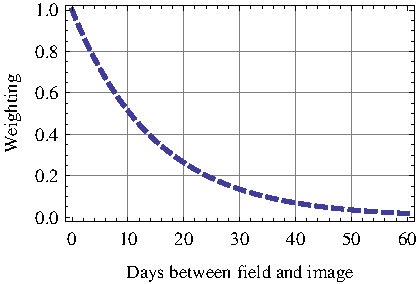
\includegraphics{dateWeightPlot.pdf}
\caption{\label{fig:dateWeighting}Site Date Difference Weighting}
\end{figure} 

\begin{figure}
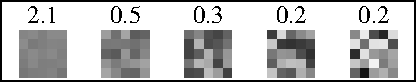
\includegraphics{homoWeightPlot.pdf}
\caption{\label{fig:varWeighting}Example site Variance Weighting} 
\end{figure} 

 \subsection{Generating Endmembers from Field Observations}

\citep{Settle1996} examined the relationship between the {}``classical'' and {}``inverse'' models for estimating cover proportions. and showed that the difference between the two estimators is less than the prediction error when mixing is linear and signatures are well separated. The classical estimator is based on a physical linear mixture model that estimates the signal produced by a mixed pixel through the use of a so-called endmenbers. \ref{eq:classicalEstimator} has the multispectral signal $x$ with $b$ spectral bands modeled as a linear function of the $c$ ground cover proportions $f$:

\begin{equation} x=Mf+\epsilon\label{eq:classicalEstimator}\end{equation} 

where $M$ is a $(b\times c)$ matrix with $c$ endmember spectra. The random noise term $\epsilon$ is assumed to be independant of $f$ and to have zero mean. That is:

\begin{equation} \varepsilon\sim N(0,\sigma^{2}I)\label{eq:whiteNoise}\end{equation} 

where $I$ is the identity matrix and $\sigma^{2}$is the noise variance. This is one of the most widely used unmixing models and has been used in a large number of research and operational projects e.g.\citep{Phinn2002a,Roeder2008a,Scarth2000}. It relies on the endmember spectra being linearly independent so that M is of full rank and invertable. 

The inverse estimator relies on a linear regression of fractional cover against the multispectral signal and has also been applied successfully in many studies e.g. \citep{Larsson1993,Williamson1993,Danaher2004,Fernandes2004}. This estimator has the form of \ref{eq:inverseEstimator}

\begin{equation} f=Ax+a\label{eq:inverseEstimator}\end{equation} 

where $(c\times b)$ matrix $A$ and $(c\times1)$ vector $a$ are calculated from the training data using multivariate regression techniques \citep{Kalivas1999}. However this method relies on having a sufficiently variable training data set that adequatly captures the landscape hetrogenaity \citep{Eldeiry2008,Salvador1998} and also requires that $X$, the $(b\times m)$ matrix of multispectral observations corresponding to the $m$ field sites has sufficient rank to allow estimation of $A$ \citep{Xu1998}. This inverse estimator has been shown to be a regularized form of the classical estimator under the assumption of linear mixing\citep{Settle1998}.
% * <rebecca.trevithick@gmail.com> 2015-01-05T04:30:10.862Z:
%
%  is there a 'b' reference for this author?
%

The inverse estimator thus allows us to invert the field data set to derive a set of endmembers by regressing the Landsat data against the field data set and then inverting the multiple regression results. Using this method, we can utilise many of the advantages of multiple regression models, such as including weighting in the regression relationship and allowing the inclusion of interactive terms which will help to model nonlinearities within the system \citep{Puyou-Lascassies1994b}. The derived endmembers can then be used in a constrained mixture analysis to improve its ability to adtapt to and model areas outside the range of calibration \citep{Phinn2002a}. 

\subsubsection{Inverting the Field Observations}

Given a field data represented as a$(c\times m)$ matrix $F$ of field cover observations and $X$ as the $([b+1]\times m)$ matrix of multispectral data where the last row is a $(m\times1)$ row of ones used to model the intercept vector $a$ from \ref{eq:inverseEstimator}we can say:

\begin{equation} F=AX\label{eq:matrixInverseEstimator}\end{equation} 

from which we can recover A using inversion techniques. The least square estimate is typically given as \citep{Lawson1995}:

\begin{equation} A=(X^{T}X)^{-1}X^{T}F\label{eq:leastSquaresSolution}\end{equation} 

However, in this work we use truncated singular value decomposition \citep{Xu1998} so that the inversion can be performed in a lower-dimensional subspace which is inportant if we are to attempt to model some of the nonlinaarities using variable transforms. Denoting $X^{+}$as the Moore\textendash{}Penrose pseudoinverse, we can recover a least squares approximation to A by inversion of \ref{eq:matrixInverseEstimator} as follows:

\begin{equation} A\approx(X^{+}F)\label{eq:invertMultispectral}\end{equation} 

We can also incorporate weighting into \ref{eq:invertMultispectral} using the standard methods for least squares. If we have a weight vector $w$ and define $X^{'}=wX$ and $F'=wF$ then \ref{eq:invertMultispectral} can be written as:

\begin{equation} A\approx(X^{'+}F^{'})\label{eq:weightedInverseMultispectral}\end{equation} 

Since we are interested in using the classical estimator From the analysis provided by \citep{Settle1998} we can compute the Moore\textendash{}Penrose pseudoinverse $A$, obtained from \ref{eq:invertMultispectral} or \ref{eq:weightedInverseMultispectral}to obtain an estimate of $M$:

\begin{equation} M\approx A^{+}\approx(X^{+}F)^{+}\label{eq:recoverEndmembers}\end{equation} 

Note that this is a different result to inverting \ref{eq:classicalEstimator} directly such that:

\begin{equation} M\approx XF^{+}\label{eq:invertClassicalEstimator}\end{equation} since in this case we are assuming that the multispectral data is the independent variable. The validity and applicability of this estimate of the endmembers is hightly dependent on having adequate field data that spans the range of cover amounts and their inherent spectral variability and also relies on a judicious choice of subspace for the inversion \citep{Elden2004}. This estimate of the endmenbers can then be used in a constrained unmixing model. It is important to note that unconstrained unmixing using the estimate of $M$ is essentially identical to unmixing directly using \ref{eq:leastSquaresSolution}. However we can use the estimate of $M$ in a constrained approach which has significant advantages when a extrapolative ability is required. 

\subsubsection{Variable Transformation and Cross Validation}

Some of the major difficulties encountered using simple linear unmixing are due to the presence of nonlinear effects which can cause model estimation errors. Since nonlinear spectral mixing occurs due to multiple reflection and transmission from surfaces \citep{Borel1994} it is particularly apparent in arid scenes where there is a bright background component, such as bright sandy soils and/or bright senescent vegetation \citep{Okin2001,Ray1996}. Since much of Queensland in the dry months is covered in senescent vegetation and there are large tracts of very bright soils in the western regions is vitally important to take account of nonlinear mixing. In this work we account for mild nonlinearities by the inclusion of log transform interactive components in the regression equations \citep{Lawrence1998}, with the use of the log transform helping to to linearise multiplicative interactions.

However one of the major problems however when using interactive terms and transformed variables in models is the ease with which an over-fitted model may be created leading to artificially inflated results and large estimation errors when used outside its calibration \citep{Salvador1998}. Some common ways of dealing with this are by using stepwise regression methods where only the best explanitory subset variables are chosen \citep{Grossman1996}, or by subspace truncation methods such as principal component regression, partial least squares or ridge regression \citep{Kalivas1999}. This study used a subspace truncation method with the truncation value being chosen using a ten-fold cross validation approach. 

\subsection{Unmixing Methodology}

There are several different ways the classical estimator \ref{eq:classicalEstimator} can be specified to solve the inverse problem to recover the fractional amount of the endmember components from the spectral information in the pixel\citep{Keshava2002}. In this work, we introduce constraints into the fractions such that$\sum_{i=1}^{c}f_{i}=1$ is a constraint such that the fractions must sum to 100\%, and $f\geq0$which constrains the fractions to be non-negative. Direct solutions are available for both the unconstrained equation and the sum to one constraint \citep{Lawson1995}. To solve the non-negative least squares (NNLS) problem a widely used algorithm is an iterative active set strategy by Lawson and Hanson \citep{Lawson1995}. To solve for both constraints we use a NNLS algorithm with a weighting strategy for the sum to one constraint that optimizes the least squares error \citep{Heinz2001}. We do this by modifing \ref{eq:classicalEstimator} so that we solve:

\begin{equation} \left[\begin{array}{c} x\\ \delta\end{array}\right]=\left[\begin{array}{c} M\\ \delta1^{T}\end{array}\right]f+\epsilon\label{eq:classicalConstrained}\end{equation} 

where $\delta$ is a weighting for the sum to one constraint and $1^{T}=\left[\begin{array}{cccc} 1 & 1 & \cdots & 1\end{array}\right]$ is a $c+1$vector of ones. The optimal value of $\delta$ is determined during the 10-fold cross validation process used to determine the subspace dimensionality of the problem. 

\subsubsection{Application to Real Imagery}

The Remote Sensing Centre work in an operational environment and has in the order of 150000 Landsat TM and ETM images on its file store. For coding simplicity, functionality and the ability to rapidly reuse scripts, the RSC used the Python programming language for the bulk of its processing needs. This has the advantage of being open source, easy to teach and can be used efficiently in a cross-platform grid computing environment. The solution of \ref{eq:classicalConstrained} currently relies on the SciPy \citep{Jones2001} wrapped version of the original FORTRAN nonlinear least squares routine by Lawson and Hansen \citep{Lawson1995}. There is however a more efficient implementation of this routine and this will be used in future implementations to speed up the computation \citep{Bro1997}. Currently it takes approximately 2 hours to process one full Landsat scene and is expected that this would halve through the use of the alternative routine. 
% * <rebecca.trevithick@gmail.com> 2015-01-06T00:26:11.278Z:
%
%  update this 5000 figure
%
% ^ <rebecca.trevithick@gmail.com> 2015-01-06T22:57:28.982Z.



\subsection{Validation using Field Data}

To test the performance of the algorithm it was applied to a timeseries of 189 Landsat TM and ETM images corresponding to WRS Path 95 and Rows 73 and 74. This part of Queensland has a large variety of cover types and has a number of long term field sites suitable for validation including the Wambiana grazing trial \citep{O'Reagain2009}, and a number of the Remote Sensing centre's Lidar transects \citep{Armston2009}. This independent field data set was used to calibrate and validate the RSC foliage projective cover product and is a primary validation source since the data were collected in identical manner to the existing fractional cover field data. These sites have moderate overstory vegetation, ranging from 0 to 30\% FPC, and so can be used to check how well the canopy affects are being modeled and removed. Over these sites the mean cover values over a 3 x 3 pixel area, centred on the field site, were compared with the field collected data. The Wambiana grazing trial in North Queensland consists of a timeseries of data over a ten-year period collected over 10 paddocks with different grazing strategies. Here, the mean cover value averaged across the entire paddock was compared with the mean of the field observed cover values after they had been transformed to objective cover estimates using the relationships from \citep{Murphy2002}. 

%%%%%%%%%%%%%%%%%%%%%%%%%%%%%%%%%%%%%%%%%%

\section{Results and Discussion}

\subsection{Field Data}

After the initial extraction, the 1549 extracted data points were visualised to check patterns, anomalies and relationships with soil colour. The data was visualised interactively in three-dimensional space, however here we will refer to figure \ref{fig:SpecCrossPlots}, which represents cross plots in the Landsat band three (red) and band four (near infrared) spectral space. The data ready to these plots is coloured according to a rainbow colour scale where red indicates values close to 100\% and violet indicates values close to 0\%. The data spread clearly shows the existence of a soil line. The plot of green cover displays the familiar triangular convex hull with the high green cover values standing out perpendicular to the soil line. However it is clear from this graph that we have collected very few high green cover sites and this may cause limitations in modelling sites with high green cover values such as cropping areas or coastal environments. The plot showing the proportional noted that cover does not display the same amount of structure is the green cover. However it is apparent that high amounts of dead cover generally correspond to low values in the red -- near infrared space. The picture is somewhat more confusing when looking at the bare ground plot as here is apparent that high amounts of bare ground in general correspond to very bright areas with high values in the red in -- near infrared space but there are also some highly bare areas with very low reflectance values. In general these correspond to very dark soil areas in the landscape. The soil colour that was recorded on each site is represented in the last plot. The colours here correspond to an RGB representation of the soil month saw colour value was recorded in the field and show quite clearly that these sites with very low red -- near infrared values correspond to black soil regions and can be seen that in general a lighter soil colour corresponds to a brighter or more highly reflective response. This plot also demonstrates that the field sites cover a large spectrum of soil colour is from very bright to very dark with many shades of red soils.

\begin{figure}
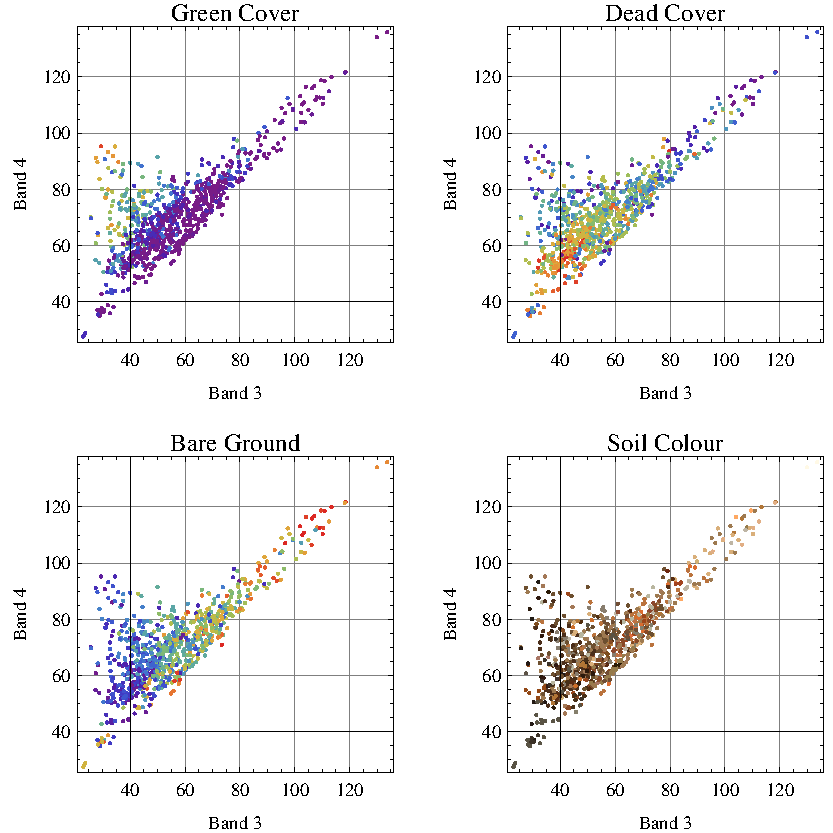
\includegraphics{bandPlots.pdf}
\caption{\label{fig:SpecCrossPlots}Cospectral plots of Landsat bands three and four with the relative amounts of the four colour types. }
\end{figure} 

 \subsection{Endmembers}

% * <rebecca.trevithick@gmail.com> 2015-01-05T04:37:40.812Z:
%
%  (Need to \underbar{maybe} add in section about how I split the field data based on albedo to generate a slightly more optimal 4-endmember set) 
%
The endmembers produced as a result of the inverse and classical equations in both transformed and transforms space were initially visually checked from anomalies and then assessed against the field data for their modelling performance.



\subsubsection{Extracted Linear Endmembers}

Figure \ref{fig:inversionMethodPlots} shows the linear end members extracted from inversion of the classical estimator, the inverse estimator, and be weighted inverse estimator. There is a large degree of similarity between three plots however the overall magnitudes of the three endmembers differs slightly between each of the plots. The bare ground and nonphotosynthetic vegetation end members that result from the inversion of the classical is estimator show a high degree of similarity in shape but are simply offset from another except in band to where there is a slight shape change. In addition, the photosynthetic vegetation shape and magnitude is very close to the nonphotosynthetic shape in magnitude. This is primarily due to the field data sampling at dry times of the year and thus not collecting sufficient amounts of green vegetation so that when the matrix of field observations is inverted there is a high degree of linear dependence on this results in a less than optimal endmember matrix. 
The end members that are derived from the inversion of the inverse estimator are very similar and, compared to the classical estimator, display less linear dependence in the Landsat bands and thus a more readily used in a least squares unmixing routine. The major difference between the weighted and non-weighted and members can be seen in the photosynthetic vegetation endmember which becomes significantly brighter when the weighting is included. The reason for this is due to the type of green colour that has been sampled on the majority of our field sampling sites. As we sample mainly in the dry time of year the presence of green cover generally were indicates that there has been a recent rainfall event. In a grassland in woodland environments of eastern Australia this green cover can change very rapidly and can also be quite patchy depending upon the antecedent conditions prior to the rainfall. Thus the weighting which considers both the time between the sensor acquisition and the field data as well as the overall site heterogeneity will have a large influence on the green endmember fraction. Given the lack of highly green sites as indicated in figure \ref{fig:SpecCrossPlots} it could be recently expected that the band four response in particular will be significantly higher once more green sites are included. This does mean however that the matter of green cover could well be being systematically overreported using the current model in areas that are dominated by photosynthetic rather than non-photosynthetic cover.

\begin{figure}
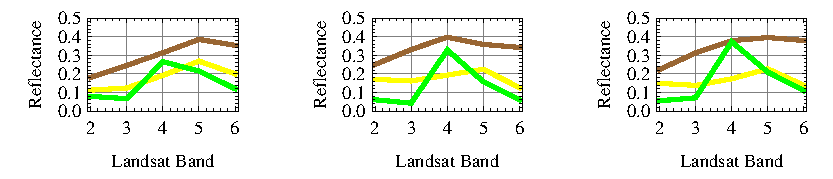
\includegraphics{methodsPlot.pdf}
\caption{\label{fig:inversionMethodPlots}Endmembers representing bare ground (brown), photosynthetic vegetation (green) and non-photosynthetic vegetation (yellow) corresponding to (from left to right): The estimates derived from the inversion of the classical estimator \ref{eq:invertClassicalEstimator}, inversion of the inverse estimator \ref{eq:recoverEndmembers}, and inversion of the inverse estimator when the field data was weighted according to \ref{eq:classicalConstrained}.}

\end{figure} 

The final set of and members derived from the weighted inverse estimator were then used to unmixed the image data corresponding to the field data sites with the varying gamma corresponding to the sum to one weight in equation \ref{eq:classicalConstrained}. The results, seen in figure \ref{fig:sum2one}, show clearly that the inclusion of a sum to one constraint improve the overall RMSE by 1\% and that the optimal value of this (in Landsat DN space) is around 50. It is interesting to note that the root mean square error then starts to get worse as the value increases, with this being due to the nonnegative least squares routine then attempting to fit the sum to one constraint more highly than fitting the spectral data itself.


\begin{figure}
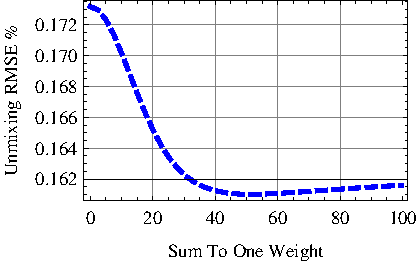
\includegraphics{sumToOnePlot.pdf}
\caption{\label{fig:sum2one}Unmixing RMSE for the 1549 field samples points vs. linear sum to one weight in the constrained unmixing model using the endmembers shown in \ref{fig:inversionMethodPlots} right panel.}
\end{figure} 

The result of using the five band Landsat linear end members with an optimised sum to one constraint is seen in figure \ref{fig:linearFit}. It can be clearly seen that the majority of the green points are clustered around the 0 to 20\% cover level and that they appear to be being over predicted by the model. The overall RMSE is 16.1\% which is a reasonable fit for a three endmember statewide model but not sufficient for operational use by management agencies and landholders. The presence of large outliers, particularly a large number of over predicted dead cover values and a large number of under predicted bare ground values means that user confidence in the produced map products would not be high.

\begin{figure}
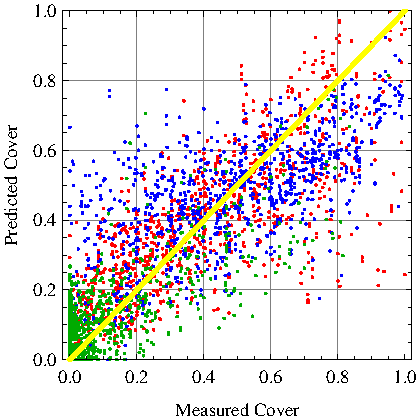
\includegraphics{linearFitPlot.pdf}

\caption{\label{fig:linearFit}Unmixing results from the untransformed model showing the fit of the bare (red), dead (blue) and green (green) components. This model had a RMSE of 16.1\% and a $r^{2}$of 0.672 (t=24, p=0.000).}

\end{figure} 

Is therefore clear that a three endmember linear model is insufficient for producing statewide scale fractional ground cover estimates however it appears that the end members are being produced through the inversion of the estimators are reasonable and a similar to endmembers that could be derived from the imagery itself. However these endmembers have the advantage of being reproducible and applicable across a large number of Landsat scenes in a large number of environments and result in a statistically highly significant model. 

\subsubsection{Final Endmembers with Variable Transformation}

Performing a logarithmic transform on the five Landsat bands followed by computing the interactive terms between or variables resulted in 55 synthetic spectral bands many of which displayed a high level of correlation with other bands. It was therefore necessary to use cross validation to attempt to recover the optimal subspace is well as the optimal sum to one constraint. The results of the cross validation can be seen in figure \ref{fig:sum2oneNL} and \ref{fig:xValidationSVs}. 

It can be seen in figure \ref{fig:sum2oneNL} that there is very little difference between having no sum to one constraint and a sum to one constraint of the optimal value of 0.2. However it must be remembered that this is indicating that the unconstrained model fits the field data very well. The sum to one constraint becomes important is when the model is asked to predict outside the region characterised by training data. When the model is being used in extrapolative sense is expected that the sum to one constraint then becomes quite important in constraining the range of values in the model solution to physically acceptable values. However it can be seen that with constrain values higher than about 0.4 the error increases significantly indicating that there is a limit as to how tightly you can expect the model to be constrained to equal 100\%

\begin{figure} 

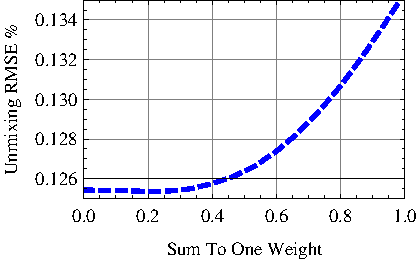
\includegraphics{sumToOnePlotNL.pdf}\caption{\label{fig:sum2oneNL}Unmixing RMSE for the 1549 field samples points vs. linear sum to one weight in the constrained unmixing model using endmembers derived using variable transformations.} 

 \end{figure} 

There is also a reasonably clear minima in figure \ref{fig:xValidationSVs} highlighting the optimal number of singular values used in the inversion. The actual minimum point itself is with 11 singular values although there is minimal difference in the root mean square error between eight and 13 singular values. This is significantly larger than the dimensionality of the original input Landsat data set and clearly shows that by adding in interactive terms we are modelling some nonlinearities within the Landsat for subspace which therefore increases the dimensionality of the data which we had to work with. It also clearly displays the effects that come from overfitting the problem when the dimensionality is increased beyond 19.

\begin{figure} 

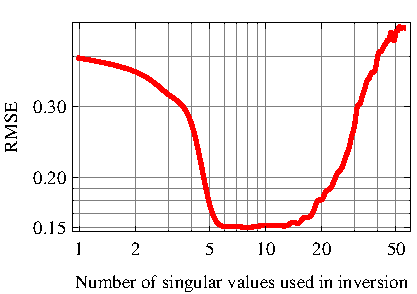
\includegraphics{xValPlotPlot.pdf}\caption{\label{fig:xValidationSVs}Selection of optimal subspace by comparing RMSE of unmixing results in 10-Fold cross validation. Lowest RMSE occurs } 

 \end{figure} 

The final model would be optimised to sum to one constraint inverted in a subspace equal to 11 dimensions resulted in the unmixing results shown in figure \ref{fig:xValidationSVs}. This final model has a root mean square error of 11.8\% and a squared Pearson product moment correlation coefficient of 0.82. This is a highly significant result indicating that the model fits extremely well in the overall root mean square error is within acceptable bounds for use in government reporting and by landholders. Compared with the linear fit there are far fewer severe outlines and also appears that the green fraction is being modelled better by the nonlinear model. Given these results the model can be applied across all Landsat scenes from where the calibration was derived and there is reasonable confidence that it will give acceptable results when used in an extrapolated scenes on land types that are found within the region.

\begin{figure}
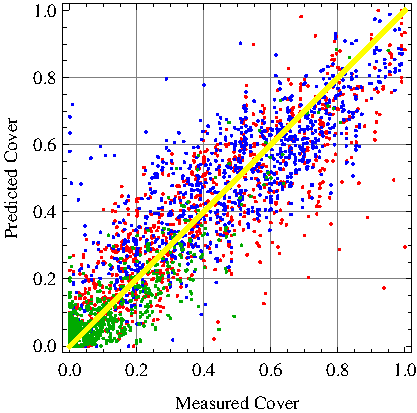
\includegraphics{nonLinearFitPlot.pdf}

\caption{\label{fig:nonLinearFit}Unmixing results from the transformed model with interactive terms showing the fit of the bare (red), dead (blue) and green (green) components. This model had a RMSE of 11.8\% and a $r^{2}$of 0.82 (t=36, p=0.0000)}

\end{figure} 



 \subsubsection{Fraction Images from the Constrained Model}

When the final model was applied to actual Landsat scenes the results were visually interpreted by operators with knowledge over these landscapes. Figure \ref{fig:imageUnmixed} shows a heterogeneity landscape where there are extremely black dark cropping soils, crops grown in both square and centre pivot irrigation systems as well as areas of grazing and some natural woodland environments to the east of the image. The fraction image is clearly picking up the variation between the bare photosynthetic and non-photosynthetic components within the imagery. The active cropping areas and the riparian areas are showing up very clearly and woodland areas or show showing up with a greater photosynthetic response. The bare dark soils in the south-west of the scene are being displayed as highly bare although there are some evidence of a slight amount of photosynthetic vegetation as indicated by some orange areas in the fraction image. Towards the middle of the scene the variation in cover levels across different paddocks can be clearly seen. Image statistics indicate that there are no negative pixels and that 99.3\% of all pixels within the image add up to 100\%$\pm$10\%. Therefore the nonnegative least squares algorithm employed in this study is producing readily interpretable results with physically realistic and qualitative endmember values.

\begin{figure}
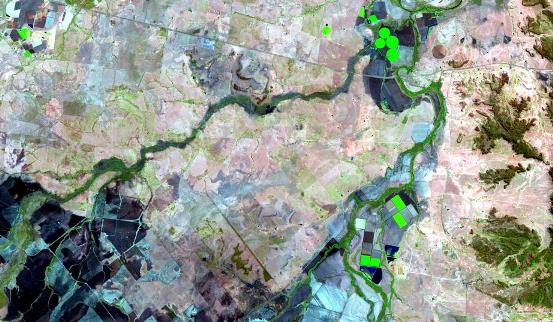
\includegraphics{l5tmre_emer_20040820_ba8m5.jpg}

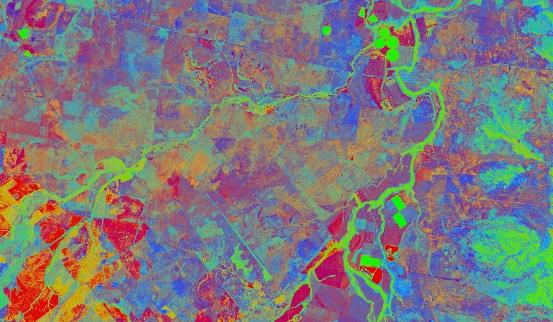
\includegraphics{l5tmre_emer_20040820_biam5.jpg}
% * <rebecca.trevithick@gmail.com> 2015-01-06T22:42:30.029Z:
%
%  want a legend?
%
\caption{\label{fig:imageUnmixed}Portion of a Landsat ETM scene near Emerald, Queensland in bands 5,4,3 as RGB and below, a fraction image of the same area with bare ground, photosynthetic vegetation and non-photosynthetic vegetation as RGB.}

\end{figure} 

\subsection{Quantitative Validation} 

\subsubsection{Validation against Lidar Sites}

\textbf{Need to pull in the field site data here }

\subsubsection{Validation at Wambiana}

The comparison between the transformed field estimated cover values and the sum of the landsat PV and NPV components measured over 10 paddocks at six monthly intervals shows a strong and consistent relationship with a close to 1:1 relationship and an RMSE of 7.2\% This result highlights the utility of satellite data to provide consistent, objective time series estimates.

\begin{figure} 

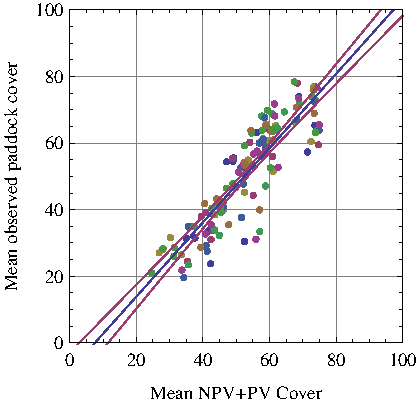
\includegraphics{wambianaComparePlot.pdf}
\caption{\label{fig:wambianaCoverCompare}This model had a RMSE of 7.2\% and a $r^{2}$of 0.78 (n=136, p=0.0000)} 

\end{figure} 

%%%%%%%%%%%%%%%%%%%%%%%%%%%%%%%%%%%%%%%%%%

\section{Conclusions}

This work has demonstrated how a network of field sites and imagery can be used to develop a robust statewide scale fractional cover model that successfully retrieves qualitative estimates of photosynthetic, non-photosynthetic and bare ground fractions. By inverting the multiple linear regression estimates and using these synthetic end members in a constrained nonnegative least squares unmixing model we have been able to successfully retrieve the cover fractions over a large number of scenes across Queensland and New South Wales, Australia.
Through the use of variable transforms and interactive terms it has been possible to model a very wide range of different surface types with a simple three endmember model. This is convenient since we seek to use these estimates in timeseries analyses, so the use of a more complex model with a greater number of endmembers would require a ruleset to apportion the endmember fractions back to the PV, NPV and bare ground cover. This work thus supports the work of \citep{Small2004a} by demonstrating that a three dimensional spectral mixing space is sufficient to model surface reflectance in most cases. It is important to note that the inclusion of a shade fraction was not necessary in this case, and had the potential to make the retrieval of the cover fractions much less accurate.
\textbf{One of the important outputs from this project was the ability to get more accurate estimates of groundcover underneath woodland canopies. By tracking the timeseries minimum and using this to adjust the ground surface fractional model we have successfully retrieved estimates of groundcover underneath moderately dense tree canopies. This work has meant that we can retrieve valid ground cover estimates over a much larger range of sites than we were previously able to using the previous index based cover system\citep{Karfs2009}. There is hope also that this method will be able to more clearly define highly bare areas under tree canopies which might correspond to active galley systems. These areas are suspected to significantly contribute to the sediment loads leading into the Great Barrier Reef that have been extremely difficult to quantify in the past. Future work will attempt to link these sub canopy ground cover estimates with regional Gully prediction models \citep{Eustace2009} to further improve the water quality modelling in these important catchments. Further work is also underway to ascertain how well this process works under moderate to very dense canopies with foliage projective cover values from 40 up to 80\%. Due to the limited field data collection in very green environments and that multiple scattering can be expected in these types environments it is expected that the retrieval will be difficult. However, in future work we will link the field datasets derived from foliage monitoring programs along with additional field data collected over very green cropping environments to further improve the model in these types environments.}

Another finding from this work was that the blue band of the Landsat sensor appears to offer considerable scope for improving performance of this unmixing algorithm. This is not entirely unsurprising since the addition of extra bands increases the dimensionality of the dataset. However the model that we propose did not use the blue band of Landsat due to the lack of an operational atmospheric correction algorithm which works consistently and reliably over the semiarid landscapes. The major limitation appears to be being able to achieve a consistent and accurate aerosol optical depth measurement in areas without significant amounts of vegetation. Work is currently underway to develop a climatology coupled with the detection of anomalous high AOD areas in the hope that in most cases the imagery would simply be corrected with a climatological aerosol value except in the case where something seems strange.

The outputs of this process are being used in operational monitoring by state and national government agencies and by individual landholders since the results of the three component model can be relatively easily understood and used in a variety of reporting contexts.\textbf{ Although successful in modelling a large range of cover types in Queensland and New South Wales environments, it is still not known how well this model would extrapolate across Australia or indeed in other countries. Considerable validation effort is needed to establish the utility of fractional cover models across different landscapes however it is often difficult to get synchronous field data with which to perform this type of validation. Future work will concentrate on collecting more field data over a variety of different environments along with coincident imagery to continue the calibration and validation of these products. One significant limitation of this work is that the ongoing problems with both Landsat five and Landsat seven mean that the sensor system is no longer an operational one and we are poised for a significant gap in coverage until the launch of Landsat eight therefore considerable work needs to be undertaken to determine a suitable Landsat replacement system in these semi arid environments. In separate work, Gill et al (2010?) have assessed the operational performance of other sensors as Landsat replacements and find that the limitations in the SWIR bands in many of the sensors would have significant limitations to their use in these environments.}

By using extensive field data sets to drive Landsat derived fractional cover time series, this work has improved methods to recover key indicators of rangeland condition, guiding better management decisions that lead to both environmental sustainability and economic productivity. Further work on cover time series derived from this research will work towards a greater understanding and spatialisation of the link between grazing pressure and the resilience of the grazing resource in the presence of considerable climate variability and climate change. These outputs benefit both local and national communities by delivering spatial information required by individual landholders, regional bodies, the Queensland Government under the Delbessie agreement and for key National Government reporting needs. They will also inform research on carbon dynamics in rangelands , processes of degradation and recovery and will provide definitive information on where land condition is improving or declining in rangelands lying directly adjacent to the Great Barrier Reef . 
%%%%%%%%%%%%%%%%%%%%%%%%%%%%%%%%%%%%%%%%%%

\acknowledgements{Acknowledgements}

This work was performed while the author was on the Queensland international Fellowship with the University of Trier in Germany. 

%%%%%%%%%%%%%%%%%%%%%%%%%%%%%%%%%%%%%%%%%%

\authorcontributions{Author Contributions}

Peter Scarth developed the theoretical framework and the method to derive the endmembers. Rebecca Trevithick collated field and image data and developed data extraction tools to train and validate the fractional cover model.

%%%%%%%%%%%%%%%%%%%%%%%%%%%%%%%%%%%%%%%%%%

\conflictofinterests{Conflicts of Interest}

The authors declare no conflict of interest. 

%=================================================================
% References: Variant A
%=================================================================
% Back Matter (References and Notes)
%----------------------------------------------------------
% Style and layout of the references
%\bibliographystyle{mdpi}
%\makeatletter
%\renewcommand\@biblabel[1]{#1. }
%\makeatother

%\begin{thebibliography}{999} % if there are less than 10 entries, enter a one digit number

%% Reference 1
%\bibitem{ref-journal}
%Lastname, F.; Author, T. The title of the cited article. {\em Journal Abbreviation} {\bf 2008}, {\em 10}, 142-149.

%% Reference 2
%\bibitem{ref-book}
%Lastname, F.F.; Author, T. The title of the cited contribution. In {\em The Book Title}; Editor, F., Meditor, A., Eds.; Publishing House: City, Country, 2007; pp. 32-58.

%\end{thebibliography}

%=================================================================
% References:  Variant B
%=================================================================
% Use the following option to include external BibTeX files:
\bibliography{scarthRefs}
\bibliographystyle{mdpi}

\end{document}